\documentclass{report}

\usepackage{fontspec}
\usepackage{xltxtra}
\usepackage[lithuanian]{babel}
\usepackage{indentfirst}
\usepackage[]{amsmath}
\usepackage{amsthm}
\usepackage{amsfonts}
\usepackage{alltt}
\usepackage[]{hyperref}
\usepackage[all]{hypcap}
%\usepackage{listingsutf8}

\hypersetup{pdfborder={0 0 0 0}}

\defaultfontfeatures{Mapping=tex-text}

% Numeravimo stiliaus pakeitimas.
\renewcommand{\theenumii}{\arabic{enumii}}
\renewcommand{\labelenumii}{\theenumii}
\renewcommand{\theenumiii}{\arabic{enumiii}}
\renewcommand{\labelenumiii}{\theenumiii}

% TODO Susitvarkyti su numeravimo atvaizdavimu. (nested enumerate; 
% label-ref)

\begin{document}

\begin{titlepage}

  \begin{center}

    %TODO: Perdaryti pagal pavyzdį pateiktą laboratorinių ir kursinių
    %darbų reikalavimų 35 puslapyje.

    % Puslapio viršus.
    {\Large Vilniaus universitetas\\
    Matematikos ir informatikos fakultetas\\
    Programų sistemų 2 kurso 2 grupė}\\[6.0cm]

    % Projekto pavadinimas.
    \textbf{ \LARGE „Nuotolinio mokymo mokyklos padalinio 
    organizuojančio stovyklas pažangiems moksleiviams pagalbinė darbų 
    valdymo ir skirstymo sistema“ }\\
    { \Large (Skirstytuvas)}\\[0.5cm]
    % TODO Pertvarkyti pavadinimą

    \textsc{\Large Verslo tikslų ir poreikių specifikacija }\\[4.0cm]

    \begin{minipage}[]{0.8\textwidth}
      \begin{flushright} \large
        \emph{Rengė:} \\
        Vytautas Astrauskas \\
        Vytautas Butkus \\
        Egidijus Lukauskas \\
        Ernestas Monginas
      \end{flushright}
    \end{minipage}

    \vfill

    {\large  Versija: 0.1 \\ \today }
  \end{center}
  
\end{titlepage}

\begin{abstract}
  V. Astrauskas, V. Butkus, E. Lukauskas, E. Monginas. Nuotolinio 
  mokymo mokyklos padalinio, organizuojančio stovyklas pažangiems
  moksleiviams, tikslų ir poreikių specifikacija (% TODO
  1 versija). VU MIF PS katedra, Vilnius 2010.

  Šiame darbe pateiktas kurso „Programų sistemų inžinerija“ laboratorinis
  darbas, skirtas verslo tikslų ir poreikių specifikavimui. Tai 
  pirmasis iš keturių pagal šį kursą daromų laboratorinių darbų.
  Darbas skirtas įsigilinti į užsakovo verslą, nustatyti problemas,
  grėsmes bei neišnaudotas galimybes ir nuspręsti ar įmanoma būtų
  sukurti programų sistemą, kuri padėtų spręsti šias problemas bei
  įgyvendinti neišnaudotas galimybes. Jei programų sistema gali
  pagerinti situaciją, nustatoma kokias būtent problemas ji padės spręsti
  bei kokias neišnaudotas galimybes ji padės įgyvendinti. Darbe atlikta
  verslo proceso analizė, pasiūlyta šio proceso tobulinimo strategija
  ir nustatyta kokias paslaugas turėtų teikti šią strategiją palaikanti 
  programų sistema. Atlikta sistemos įgyvendinamumo analizė bei nustatyta
  kokią konkrečią naudą ji teiks naudotojams.
  
  Informacija apie vykdytojus ir jų įnašą į darbą:

  \begin{itemize}
    \item Vytautas Astrauskas (\url{Vytautas.Astrauskas@mif.stud.vu.lt}): 
      \begin{itemize}
        \item Verslo proceso aprašas.
        \item Išorinė verslo proceso analizė.
        \item Vidinė verslo proceso analizė.
        \item Verslo tobulinimo strategija.
        \item Strateginiai ir operaciniai tikslai verslo tobulinimo
          strategijai įgyvendinti.
        \item Užsakovo poreikių analizė.
        \item Esamoji būklė.
      \end{itemize}

    \item Vytautas Butkus (\url{Vytautas.Butkus.2@mif.stud.vu.lt}): 
      \begin{itemize}
        \item Juridinis įgyvendinamumas.
        \item Sistemos panaudojimas.
        \item Sistemos teikiama nauda.
      \end{itemize}

    \item Egidijus Lukauskas (\url{Egidijus.Lukauskas@mif.stud.vu.lt}): 
      \begin{itemize}
        \item Scenarijaus aprašas.
        \item Priemonės scenarijui įgyvendinti.
      \end{itemize}

    \item Ernestas Monginas (\url{Ernestas.Monginas@mif.stud.vu.lt}):
      \begin{itemize}
        \item Operacinis įgyvendinamumas.
        \item Techninis įgyvendinamumas.
        \item Ekonominis įgyvendinamumas.
      \end{itemize}

  \end{itemize}
  
\end{abstract}


\tableofcontents

\chapter{Įvadas}

% TODO: žr. 5 reikalavimų psl.

\section{Programų sistemos pavadinimas}
% TODO

\section{Dalykinė sritis}
% TODO

\section{Probleminė sritis}
% TODO

\section{Naudotojai}
% TODO

\section{Darbo pagrindas}
% TODO

%TODO: ištrinti, kai bus normalių citatų.
Beprasmė citata iš Čaplinsko vadovėlio: „Objektinio stiliaus architektūros
grindžiamos objektine paradigma. Ji šiuo metu yra 
vyraujanti.“\cite[50]{cap_psi2}

\section{Naudoti dokumentai}
% TODO

\bibliographystyle{plain}
\bibliography{bibliography}

\chapter{Verslo proceso analizė}

\section{Verslo proceso aprašas}

Nuotolinio mokymo mokyklos padalinys, organizuojantis stovyklas pažangiems
moksleiviams, yra atsakingas už vidutiniškai dešimties dienų trukmės
stovyklos vidutiniškai šimtui moksleivių suorganizavimą. Šis padalinys
rūpinasi nurodytų, kaip pažangių, moksleivių, bei jų dėstytojų pakvietimu, 
apgyvendinimu, bei maitinimu. Taip pat jis atsakingas už stovyklos metu 
skaitomų paskaitų kokybę, bei moksleivių aprūpinimą visomis reikalingomis
darbui priemonėmis. Didžiąją dalį stovyklos organizavimui reikalingų lėšų
duoda nuotolinio mokymo mokyklos rėmėjai, o trūkumą padengia į stovyklą
važiuojantys moksleiviai, sumokėdami dalyvio mokestį. Su moksleiviais ir
dėstytojais dažniausiai bendraujama elektroniniais individualiais 
laiškais, o duomenys saugomi popieriuje, bei MS Excel skaičiatlentėse.

\section{Išorinė verslo proceso analizė}

\subsection{Analizės rezultatai}

Stovyklų organizavimo tikslas yra suteikti moksleiviams galimybę pagilinti
savo žinias ir kitaip patobulėti. Taigi pagrindinė proceso įeiga ir išeiga
yra tie patys moksleiviai. Apie į stovyklą kviečiamus moksleivius, mes
žinome, jų nuotolinio mokymosi rezultatus, bei kokia jų dalis priima 
kvietimą dalyvauti stovykloje (įeigos kriterijai). Po stovyklos
praėjus laiko tarpui, mes vėl galime įvertinti moksleivių nuotolinio
mokymosi rezultatus, be to moksleiviai užpildo įvertinimo anketas, kuriose
nurodo, kaip jiems patiko konkrečios paskaitos ir visa stovykla apskritai
(išeigos kriterijai). Taip pat organizuojant stovyklą yra svarbu jos 
organizavimo kaina (nes jai didėjant dalyvio mokestis kai kuriems 
moksleiviams gali tapti per dideliu), bei organizuojant padarytų klaidų
(nusižengimai įstatymams, susitarimams, bei darbo klaidos) kiekis.

Apibendrindami, galime išskirti tokius stovyklų organizavimo proceso 
vertinimo kriterijus:
\begin{enumerate}
  \item motyvacijos mokytis pokytis (motyvacija mokytis) – kiek padidėjo
    ar sumažėjo moksleivio teisingai išspręstų ir visų jam duotų užduočių
    santykis;
  \item moksleivių noras dalyvauti stovykloje (noras dalyvauti) – kokia 
    dalis moksleivių, gavusių kvietimą, pareiškia norą dalyvauti;
  \item moksleivių atsiliepimai apie stovyklą pasitenkinimo anketoje;
  \item stovyklos organizavimo sąnaudos (kaina);
  \item juridinių aktų (įstatymų (buhalterinės apskaitos,
    mokesčių administravimo, asmens duomenų teisinės apsaugos
    ir kiti), bei susitarimų) pažeidimų skaičius;
  \item padarytų darbinių klaidų (pavyzdžiui rėmėjo pavadinimas 
    atspausdintas su klaida, arba kvietimas išsiųstas ne tam moksleiviui, 
    kuriam reikėjo) skaičius;
  \item neištaisytų klaidų skaičius;
  \item pažeidimų  ir klaidų sukeltų padarinių vertė – kiek kainuotų juos 
    pašalinti, jei būtų bandoma tai daryti + moralinė žala;
  \item didžiausias galimas turimos komandos aptarnaujamų moksleivių 
    skaičius.
\end{enumerate}

Kriterijų detalizavimas, ir jų kritinės vertės:

\begin{tabular}[]{| l | p{2.2cm} | c |}
  \hline
  Kriterijus & Matas & Kritinė vertė \\
  \hline
  Motyvacija mokytis & Procentai & < -5\% (sumažėjo 5\%) \\
  \hline
  Noras dalyvauti & Procentai & < 80\% \\
  \hline
  Moksleivių įvertinimas & Dešimtbalė sistema & < 7 \\
  \hline
  Stovyklos kaina & Litais dalyviui & > 2000Lt \\
  \hline
  Pažeidimų skaičius & Vienetais & > 0 \\
  \hline
  Klaidų skaičius & Vienetais & \\
  \hline
  Neištaisytų klaidų skaičius & Vienetais & > 0 \\
  \hline
  Pažeidimų ir klaidų kaina & Litais & > 1000Lt \\
  \hline
  Aptarnautų moksleivių skaičius & Vienetais & < 80 \\
  \hline
\end{tabular}

\subsection{Problemos, grėsmės ir neišnaudotos galimybės}

Problemos:
\begin{itemize}
  \item Didelis paliktų neištaisytų klaidų skaičius.
\end{itemize}

Grėsmės:
\begin{itemize}
  \item Paramos gaunamos iš rėmėjų mažėjimas. 
                                        % Gali sukelti tiek populiarumo 
                                        % mažėjimas, tiek didelis klaidų
                                        % kiekis.
  \item Padidėjus stovyklos kainai, moksleiviai gali nebevažiuoti, nes 
    jiems bus per brangu.
  \item Moksleivių noro dalyvauti mažėjimas.
\end{itemize}

Neišnaudos galimybės:
\begin{itemize}
% TODO O kaip jei šio mato padidėjimas, taip pat leistų geriau aptarnauti
% esamus, nes būtų daugiau laiko įsiklausyti į jų specialiuosius 
% pageidavimus? Jei kriterijus būtų ne apskritai kiek moksleivių komanda
% yra pajėgi aptarnauti, bet kiek ji yra pajėgi pašalinti specialiųjų
% atvejų?
  \item Į stovykla pakviečiama mažiau moksleivių, negu gauta parama
    suteikia galimybę pakviesti.        % TODO Ar tai tikrai yra 
                                        % neišnaudota galimybė?
% \item Į stovykla kviečiama mažiau moksleivių nei leidžia biudžetas, nes
%   organizavimo komanda nėra pajėgi jų visų aptarnauti.
\end{itemize}

\section{Vidinė verslo proceso analizė}

Problemos:
\begin{itemize}
  \item Atlikus analizę paaiškėjo, jog tam, kad proceso vykdymo metu yra
    padaroma daug klaidų, bei tam, kad jos nėra laiku ištaisomos turi
    įtakos:
    \begin{enumerate}
      \item Visi darbai daromi rankomis. (Pavyzdžiui: nors ir kvietimai
        siunčiami elektroniniu paštu, bet jų tekstas yra renkamas ranka.)
      \item Netikėti vėlavimai atliekant proceso grandinės dalis. Dėl jų 
        negalima atlikti vėlesnių tai grandinei priklausančių darbų, nes
        jie yra nuo jos priklausomi. Dėl to paskutinę savaitę susikaupia
        darbų sankaupa, su kuria nebepajėgiama susitvarkyti.
    \end{enumerate}
\end{itemize}

Grėsmės:
\begin{itemize}
  \item Padidėjus paliktų klaidų skaičiui, rėmėjai gali nuspręsti, kad 
    stovyklos organizatoriai nėra pajėgus kokybiškai panaudoti jų pinigus
    ir todėl nutraukti finansavimą, dėl ko padidėtų dalyvavimo mokestis ir
    dalis moksleivių nebegalėtų dalyvauti.
  \item Kritus stovyklos organizavimo kokybei, gali sumažėti stovyklos
    populiarumas.
\end{itemize}

\section{Verslo tobulinimo strategija}

Pagrindinis verslo tobulinimo siekis: padidinti darbo efektyvumą ir 
sumažinti klaidų skaičių.

\section{Strateginiai ir operaciniai tikslai verslo tobulinimo %
  strategijai įgyvendinti}

Strateginiai tikslai:
\begin{enumerate}
  \item \label{tiksl_efek} Padidinti darbo efektyvumą.
    \begin{enumerate}
      \item \label{tiksl_auto} Įdiegti priemones leidžiančias automatizuoti 
        mechaninius darbus:
        \begin{enumerate}
          \item \label{tiksl_el} kvietimų moksleiviams siuntimas;
          \item \label{tiksl_r} moksleivių informacijos surinkimas.
        \end{enumerate}
    \end{enumerate}
  \item \label{tiksl_kl} Sumažinti klaidų skaičių.
    \begin{enumerate}
      \item \label{tiksl_vald} Įdiegti priemones leidžiančias efektyviai 
        sekti ir valdyti darbo eigą:
        \begin{enumerate}
          \item \label{tiksl_dvisk} vienoje vietoje matyti visų darbų 
            sąrašą, bei kaip jų vykdymas atitinka numatytąjį planą;
          \item \label{tiksl_dbus} peržiūrėti darbo būseną (negalimas 
            pradėti vykdyti, nes
            nebaigti kiti darbai nuo kurių šis priklauso; galimas pradėti
            vykdyti; pradėtas vykdyti; baigtas vykdyti; patikrintas);
          \item \label{tiksl_dinfo} peržiūrėti darbo informaciją (ką 
            konkrečiai reikia 
            atlikti; kokius darbus reikia atlikti prieš tai; kada 
            vėliausiai darbas turi būti pradėtas, kad būtų baigtas laiku;
            kiek vidutiniškai jį užtrunka atlikti; kokios dažniausiai 
            iškyla problemos jį vykdant; jei vėluoja, tai kiek);
          \item \label{tiksl_dvyk} peržiūrėti vykdytojus (kas vykdė/vykdo 
            šį darbą; kas atliko peržiūrą);
          \item \label{tiksl_dv} kiekvienas vykdytojas (jei jam suteiktos 
            tokios teisės) gali pasiimti darbą vykdymui arba peržiūrai.
                                        % XXX Rašant naudojimo scenarijų, 
                                        % nepamiršti patikrinti ar aktorius
                                        % turi reikiamas teises atlikti 
                                        % veiksmą. (Ne visiems leidžiama
                                        % dirbti su asmeniniais moksleivių
                                        % duomenimis.)
        \end{enumerate}
    \end{enumerate}
\end{enumerate}

\section{Užsakovo poreikių analizė}

% TODO Kaip daryti lenteles su LaTeX parašyta čia:
% http://en.wikibooks.org/wiki/LaTeX/Tables

\begin{tabular}[]{| l | p{1.6cm} | p{5.8cm} | c |}
  \hline
  Nr. & Operacinis tikslas & Resursai, reikalingi tikslui įgyvendinti &
  Prioritetas \\
  \hline
  1. & \ref{tiksl_el} & TODO & ? \\
  \hline
\end{tabular}

\chapter{Užsakovo poreikių analizė}

% TODO Suvesti terminus į žodynėlį.

\ref{tab:poreikiai} lentelėje pateiktas sąrašas kompiuterinių resursų, 
kurių reikia norinti įgyvendinti \emph{\nameref{section_strat_oper_tiksl}}
skyrelyje aprašytiems operaciniams tikslams.

Iš pateiktų operacinių tikslų, matome, jog siekiui įgyvendinti reikalinga
programų sistema galinti:
\begin{itemize}
  \item siųsti elektroninius laiškus;
  \item saugoti darbų sąrašus su informacija apie kiekvieną iš jų;
  \item priimti informaciją iš moksleivių.
\end{itemize}

\begin{table}
  \centering
  \begin{tabular}[]{| l | p{1.6cm} | p{5.8cm} | c |}
    \hline
    Nr. & Operacinis tikslas & Resursai, reikalingi tikslui įgyvendinti &
    Prioritetas \\
    \hline
    1. & \ref{tiksl_el} & 
      \Gls{p_serveris}; \gls{duom_baz} su moksleivių duomenimis. & 1 \\
    \hline
    2. & \ref{tiksl_r} & 
      \Gls{svetaine}, jos valdymo ir priežiūros įrankiai; 
      \gls{duom_baz} moksleivių duomenims saugoti. & 1 \\
    \hline
    3. & \ref{tiksl_dvisk} &
      \Gls{duom_baz} duomenims apie darbus saugoti. & 2 \\
    \hline
    4. & \ref{tiksl_dbus} &
      \Gls{duom_baz} duomenims apie darbus saugoti. & 2 \\
    \hline
    5. & \ref{tiksl_dinfo} &
      \Gls{duom_baz} duomenims apie darbus saugoti. & 2 \\
    \hline
    6. & \ref{tiksl_dvyk} &
      \Gls{duom_baz} duomenims apie darbus ir jų vykdytojus 
      saugoti. & 3 \\
    \hline
    7. & \ref{tiksl_dv} &
      \Gls{duom_baz} duomenims apie darbus, bei vykdytojus ir 
      jiems suteiktas teises, saugoti. & 3 \\
    \hline
    8. & \ref{tiksl_vad} &
      \Gls{duom_baz} duomenims apie darbus saugoti. & 2 \\
    \hline
  \end{tabular}
  \caption{Užsakovo poreikių analizės lentelė}
  \label{tab:poreikiai}
\end{table}


\chapter{Sistemos naudojimo scenarijus}

\section{Esamoji būklė}

Mokyklos būstinėje yra vienas nešiojamas kompiuteris su Windows operacine
sistema, kuriame laikomi visi „einamieji“ duomenys, bei prie jo prijungtas 
lazerinis spausdintuvas. Nuotolinio mokymo mokykla taip pat turi savo 
svetainę, bei duomenų bazę su informacija apie moksleivius ir dėstytojus.
Darbuotojai dirba su savo asmeniniais kompiuteriais, kuriuose naudoja
įvairią programinę įrangą (pavyzdžiui naudojamų operacinių sistemų 
sąraše yra „Windows XP“, „Windows 7“, „Ubuntu Linux“, „Xubuntu Linux“,
„Gentoo Linux“). Dauguma darbuotojų turi didelę darbo su biuro 
programomis patirtį.

\section{Scenarijaus aprašas}

\ref{fig:uml_usecase} diagramoje pavaizduota darbo su sistema UML schema.
\hfill \\

Vadovas informuoja sistemą, kad stovyklos organizavimas yra pradedamas.
Jis į sistemą įkelia darbų sąrašą, kiekvienam darbui nurodydamas atributus.
Po to         % TODO : Atributus įkelti į žodyną
prideda vykdytojus, kurie atlikinės darbus iš darbų sąrašo. Vos pridėjus
vykdytoją, sistema jį apie tai informuoja elektroniniu laišku. 

Vykdytojas prisijungęs prie
sistemos gali peržiūrėti darbų sąrašą. Jis pasirenka
darbą, kurį atlikinės. Baigęs pasirinkto darbo vykdymą, pažymi tą
darbą kaip atliktą. Sistema informuoja vadovą apie darbo atlikimą ir
paprašo tai patvirtinti. Vadovui atmetus darbo atlikimą, sistema informuoja
apie tai vykdytoją prašydama pataisyti darbą. Vykdytojui patvirtinus
apie darbo pataisymą, sistema vėl prašo vadovo patvirtinti darbo kokybę. 
Taip daroma tol, kol vadovas patvirtina darbo kokybę. 

Vėliau vadovas prideda kviečiamų moksleivių sąrašą. Sistema jiems išsiunčia
kvietimus reikalaudama patvirtinti, jog dalyvaus, arba pranešti, kad negalės 
atvykti. Patvirtinusių dalyvavimą moksleivių paprašoma patikslinti jų 
asmeninius duomenis, patvirtinti jų teisingumą. Kai užbaigiamas tvarkaraščio
sudarymo darbas, sistema nusiunčia visiems dalyvausiantiems moksleiviams
tvarkaraščio kopiją.

Pasibaigus stovyklai vadovas praneša apie tai sistemai. Ji moksleiviams
išsiuntinėja stovyklos vertinimo anketas bei darbų vykdytojų paprašo 
pateikti stovyklos raportą. Sistema, gavusi visus grįžtamuosius atsakymus,
suformuoja ataskaitą ir ją pateikia stovyklos vadovui.

\begin{figure}[htb]
  \begin{center}
    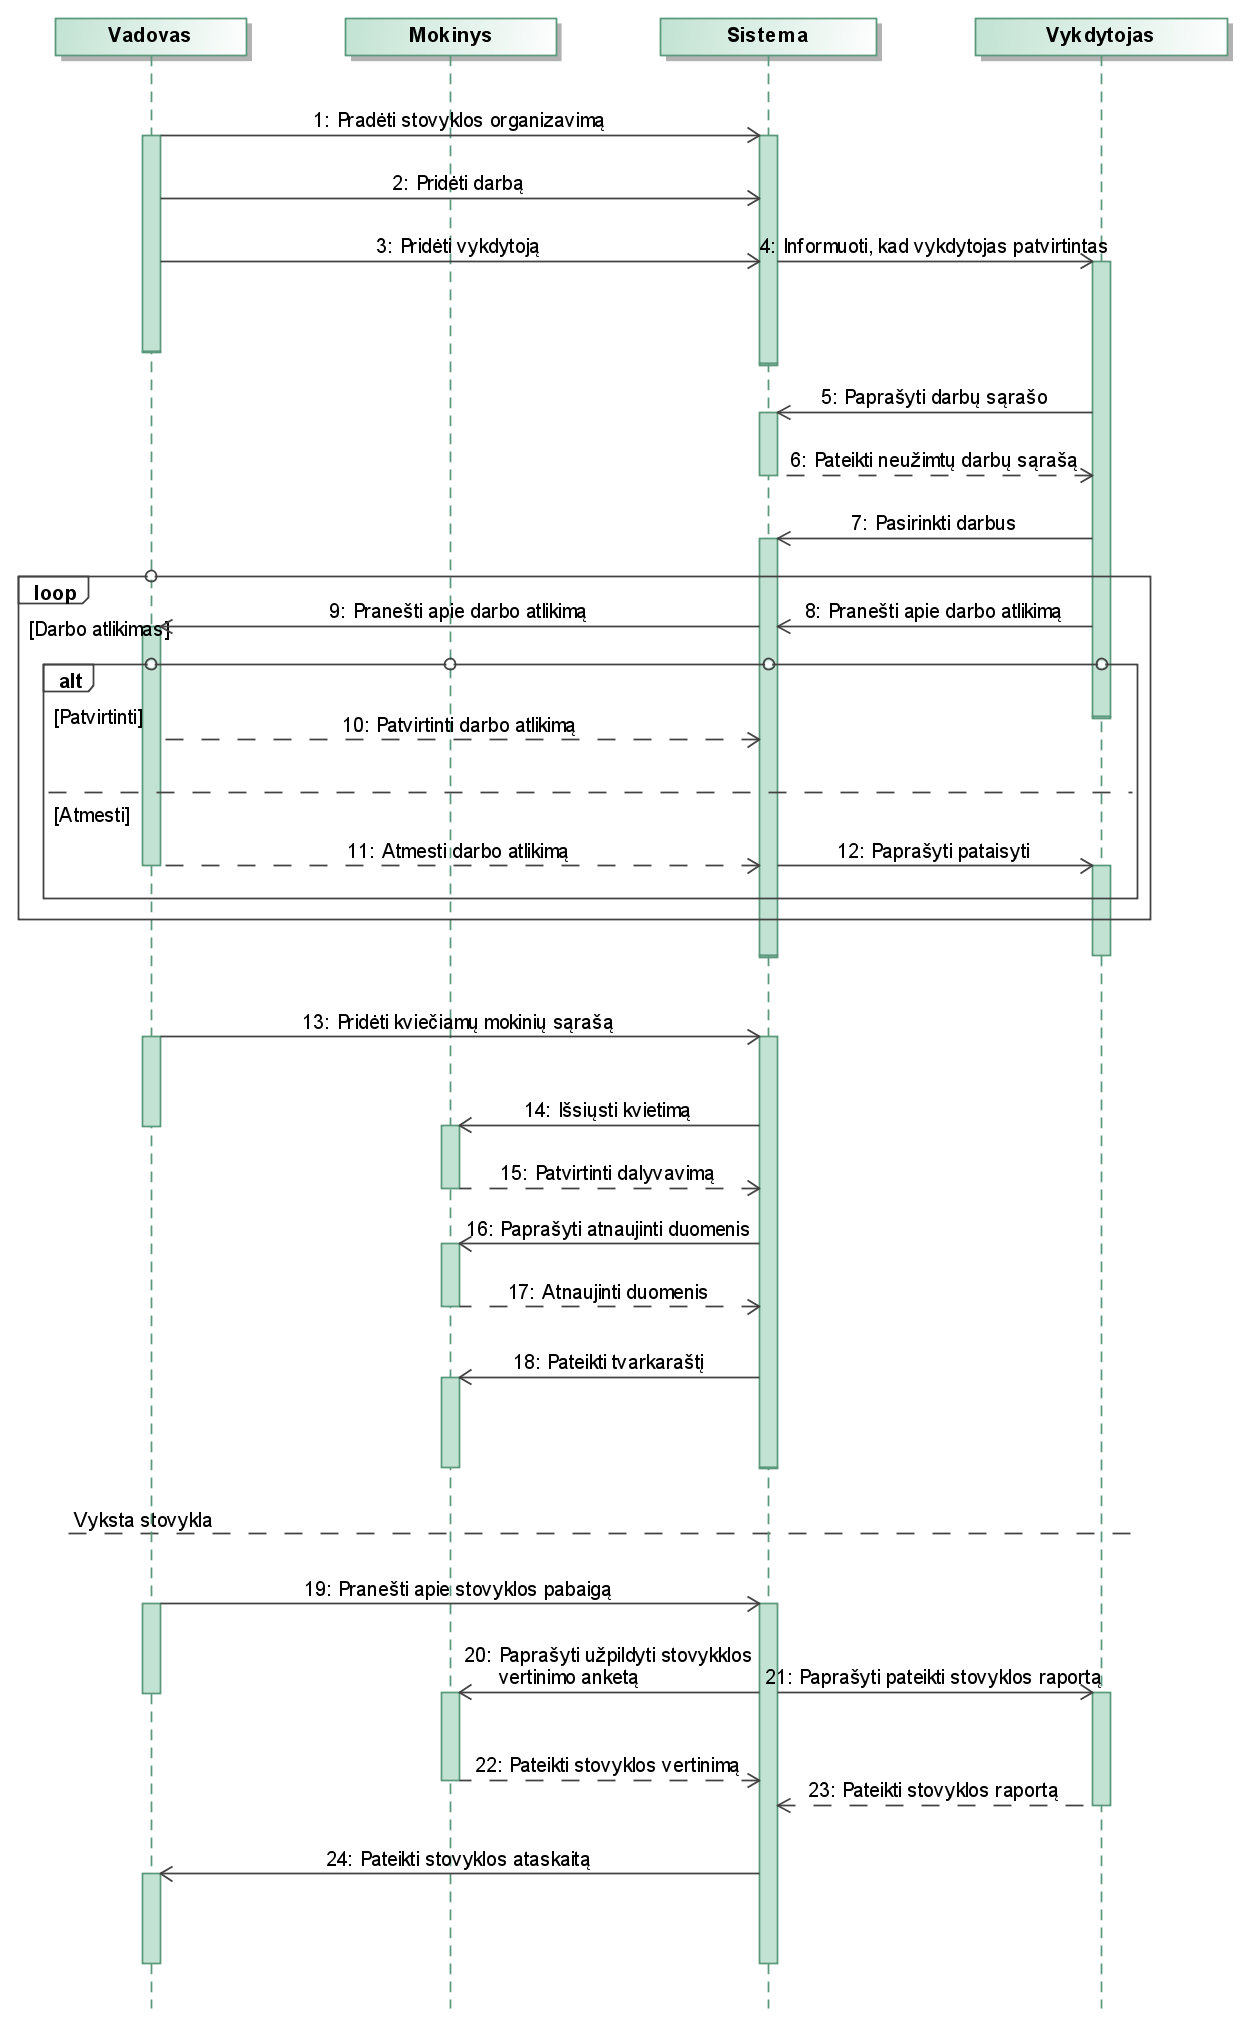
\includegraphics[scale=0.7]{images/Seka.png}
    \caption{UML schema vaizduojanti darbą su įdiegta sistema.}
  \end{center}
  \label{fig:uml_usecase}
\end{figure}


\subsection{Darbo vietų aprašas}
\begin{enumerate}
  \item \emph{Vadovas}
	\begin{itemize}
	  \item Techninė įranga:
		\begin{enumerate}
			\item kompiuteris su internetu.
		\end{enumerate}
	  \item Programinė įranga:
		\begin{enumerate}
			\item operacinė sistema;
      \item interneto naršyklė.
		\end{enumerate}
	  \item Kvalifikaciniai reikalavimai:
		\begin{enumerate}
			\item kompiuterinio raštingumo pagrindai;
			\item sistemos „Skirstytuvas“ administravimo apmokymas.
		\end{enumerate}
	\end{itemize}

  \item \emph{Vykdytojas}
	\begin{itemize}
	  \item Techninė įranga:
		\begin{enumerate}
			\item kompiuteris su internetu.
		\end{enumerate}
	  \item Programinė įranga:
		\begin{enumerate}
			\item operacinė sistema;
      \item interneto naršyklė.
		\end{enumerate}
	  \item Kvalifikaciniai reikalavimai:
		\begin{enumerate}
			\item kompiuterinio raštingumo pagrindai;
			\item sistemos „Skirstytuvas“ naudojimo apmokymas.
		\end{enumerate}
	\end{itemize}
\end{enumerate}

\section{Priemonės scenarijui įgyvendinti}
\begin{enumerate}
	\item Virtuali tarnybinė stotis
	\item Tinklo įranga
	\item Pašto serveris
	\item Duomenų bazių valdymo sistemos
	\item Interneto ryšio paslaugos
	\item Operacinės sistemos
	\item Darbuotojų apmokymas naudotis sistema
	\item Interneto svetainės vardo sritis .lt zonoje
\end{enumerate}
\chapter{Sistemos įgyvendinamumo ir teikiamos naudos analizė}

% TODO

\section{Operacinis įgyvendinamumas}

% TODO

\section{Techninis įgyvendinamums}

% TODO

\section{Ekonominis įgyvendinamumas}

% TODO

\section{Juridinis įgyvendinamumas}

Kuriama sistema neprieštarauja Lietuvos Respublikos įstatymams. Stovyklos 
dalyvių asmens duomenų rinkimas neprieštarauja Lietuvos Respublikos 
Asmens duomenų teisinės apsaugos įstatymui. Kiekvienam dalyviui bus 
suteikiama galimybė nesutikti su jo asmens duomenų rinkimu, arba davus 
leidimą peržiūrėti jau surinktus duomenis ir panorėjus juos pakeisti. 
Pasibaigus stovyklos organizavimo ir vykdymo laikotarpiui nereikalingi 
duomenys bus sunaikinami. Taip pat numatoma laikytis visų duomenų saugumo 
kriterijų.
% TODO Pridėti nuorodą į straipsnį.

\section{Sistemos panaudojimas}

\ref{fig:uml_tasks} UML schemoje vaizduojamos aktorių vykdomos užduotys ir 
kaip jas padeda vykdyti sistema.

\begin{figure}[htb]
  \begin{center}
    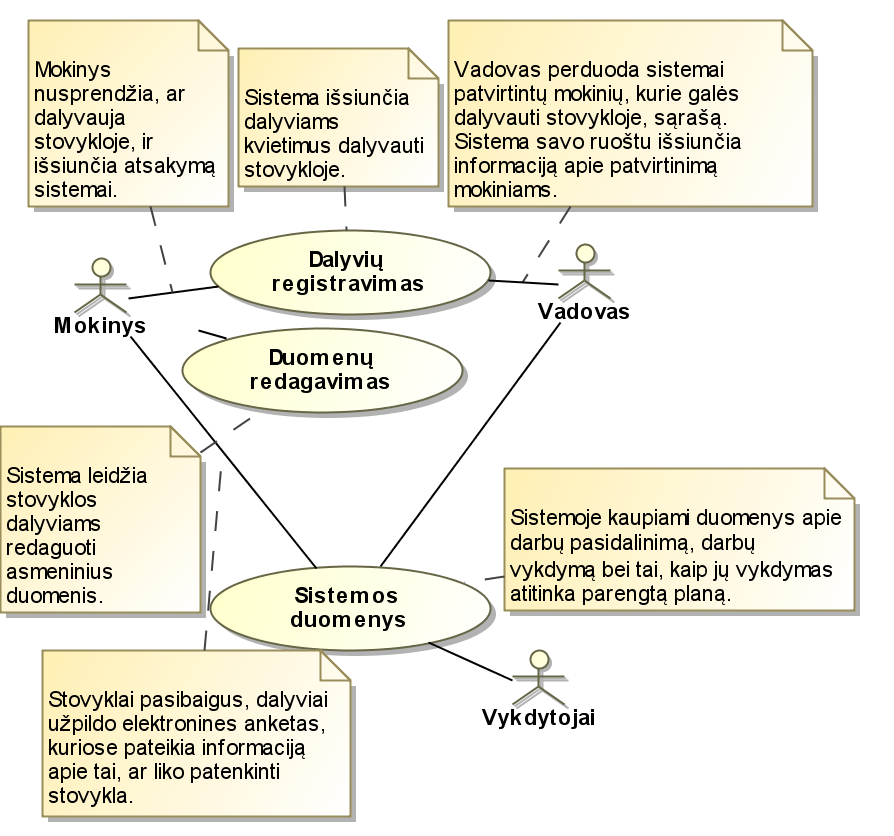
\includegraphics[scale=0.8]{images/sistemos_panaudojimas.png}
  \end{center}
  \caption{UML schema vaizduojamos aktorių vykdomos užduotys ir kaip jas
    padeda vykdyti sistema.}
  \label{fig:uml_tasks}
\end{figure}

\section{Sistemos teikiama nauda}

\ref{fig:uml_tasks2} UML schema vaizduojamos aktorių vykdomos užduotys 
ir kaip jas
padeda vykdyti sistema.

\begin{figure}[htb]
  \begin{center}
    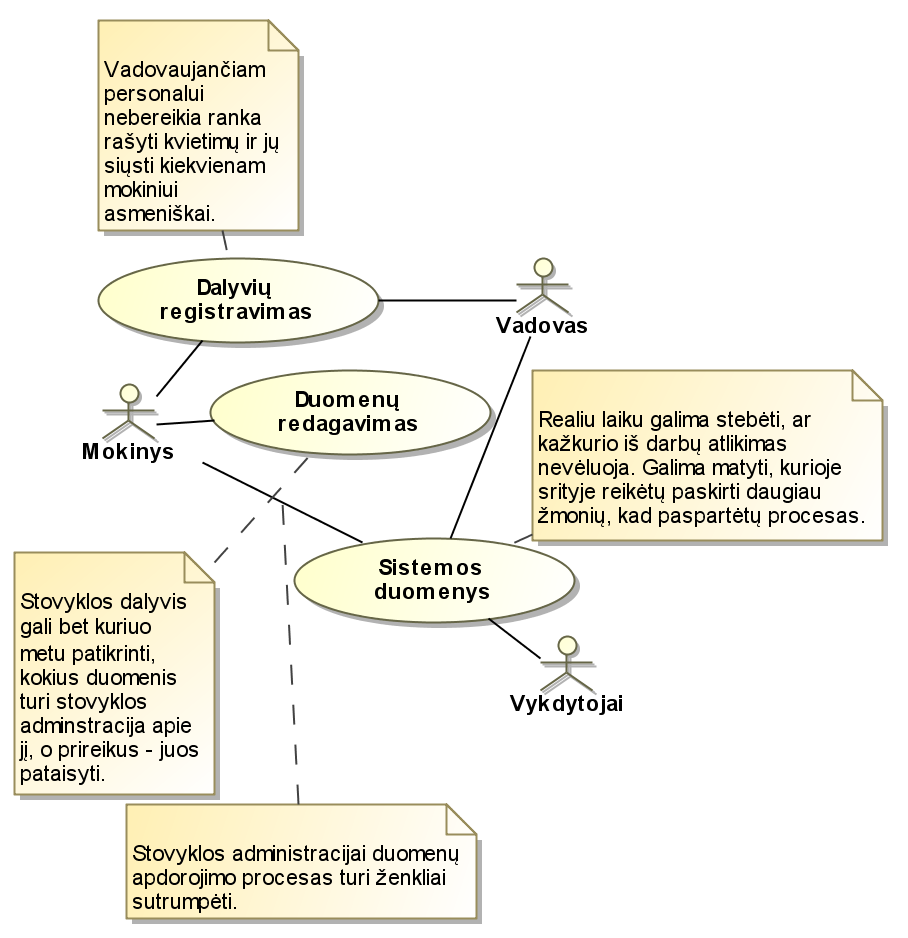
\includegraphics[scale=0.8]{images/sistemos_tiekiama_nauda.png}
  \end{center}
  \caption{UML schema vaizduojamos aktorių vykdomos užduotys ir kaip jas
    padeda vykdyti sistema.}
  \label{fig:uml_tasks2}
\end{figure}

\chapter{Išvados}

% TODO


\clearpage
\phantomsection
\addcontentsline{toc}{chapter}{Literatūra}
\bibliographystyle{plain}
\bibliography{bibliography}

\end{document}
